% Provenance (never printed): see sources/outline_sources.md (Year 1: compaction and
% cementation; basin types; subsidence, accommodation and sea-level change). Exercise and
% problem values in the Book 3 scratch calculator calc/ch23.py; figure data from
% figdata/bachelor-1/compaction.py and sea_level.py.
% Porosity and permeability are Book 1's (g6); diagenesis was met in Book 2 (g12) and is
% re-founded here; sedimentary basin was met in Book 2 (g11) and is re-founded here;
% isostasy and the equal-mass proposition are ch. 11's; passive margins and rifts ch. 13's;
% effective stress ch. 16's; the Last Glacial Maximum and glacial cycles Book 2's (g12).
% Pressure solution is defined in the Year 3 volume (deformation mechanisms): prose only.
% Backstripping, the stretching model and the comparison of basins are the Year 2 volume's.
\chapter{الدياجينيز والأحواض الرسوبية}\label{ch:b1:diagenesis-basins}

الرمل الشاطئي مفكّك: نصفه، بالحجم، ماء يملأ ما بين حبيباته. ومدفونًا على عمق ثلاثة كيلومترات، يعود الرمل نفسه في عيّنة حفر حجرًا رمليًّا صلبًا، حبيباته مضغوطة معًا، والفراغ بينها قد نقص كثيرًا وامتلأ جزئيًّا بكوارتز جديد. وبين الشاطئ والعيّنة تقع ملايين السنين، دُفن فيها الرسوب تحت رسوب أكثر، وضُغط وسُخّن وتشرّب ماء أذاب بعض \omterm{def:b1:rock-forming-minerals:mineral}{المعادن} وأرسى غيرها. يتتبّع هذا الفصل تلك التغيّرات، ثم يعود إلى الأماكن التي يمكن أن يتراكم فيها الرسوب كيلومترات في السماكة، أي \omterm{def:b1:diagenesis-basins:basin}{الأحواض الرسوبية}، وإلى الأمرين اللذين يصنعان فيها المكان: هبوط القاع، وارتفاع البحر وانخفاضه.

\begin{recall}
المسامية في الصخر هي الكسر من حجمه المكوّن من مسام، والنفاذية تقيس مدى سهولة جريان الماء فيها (الكتاب الأول، الصف السادس). وتكون منطقة في توازن إيزوستاسي حين يحمل كل عمود حتى \omterm{def:b1:isostasy-gravity:isostasy}{عمق التعويض} الكتلة نفسها (\cref{prop:b1:isostasy-gravity:equal-mass}). وتتفتّح الصدوع بالانزلاق العادي، والهوامش السلبية هي حواف القارات التي تُترك خلفها حين يصير الصدع محيطًا (\cref{ch:b1:rifts-ridges-margins}). \omterm{def:b1:stress-strain-rheology:lithostatic}{والإجهاد الفعّال} هو الإجهاد ناقص ضغط مائع المسام (\cref{def:b1:stress-strain-rheology:lithostatic}). وبلغت آخر دورة جليدية أقصى عصورها الجليدية قبل نحو عشرين ألف سنة (الكتاب الثاني، الصف الثاني عشر). والحجارة الرملية والصخور الطينية وبيئاتها هي ما في \cref{ch:b1:clastic-sediments}؛ أما الحجر الكلسي والطباشير والدولوميت \omterm{def:b1:chemical-biogenic-sediments:evaporite}{والرسوبات التبخّرية} فبيئاتها في \cref{ch:b1:chemical-biogenic-sediments}.
\end{recall}

\section{الانضغاط}\label{sec:b1:diagenesis-basins:compaction}

الرسوب الجديد رصٌّ مفكّك للحبيبات مع ماء بينها. وكل ما يحدث له بعد الترسيب وقبل التحوّل الصخري، وهو يبقى عند درجات الحرارة والضغوط المنخفضة في أعلى بضعة كيلومترات من \omterm{def:b1:layered-earth:layers}{القشرة}، ينتمي إلى عائلة واحدة من العمليات.

\begin{definition}[الدياجينيز]\label{def:b1:diagenesis-basins:diagenesis}
\emph{الدياجينيز}\index{الدياجينيز} هو مجموعة التغيّرات الفيزيائية والكيميائية والحيوية التي يمرّ بها الرسوب بعد ترسيبه، عند درجات حرارة وضغوط \omterm{def:b1:layered-earth:layers}{القشرة} العليا، دون ضغوط التحوّل الصخري ودرجاته. ويشمل \omterm{def:b1:diagenesis-basins:compaction}{الانضغاط}، \omterm{def:b1:diagenesis-basins:cement}{والتلحيم}، وانحلال الحبيبات، وإحلال \omterm{def:b1:rock-forming-minerals:mineral}{معدن} محلّ آخر؛ وتحوّل هذه كلّها معًا الرسوب المفكّك إلى صخر رسوبي.
\end{definition}

أول هذه التغيّرات ميكانيكية. فكل طبقة جديدة تضيف وزنها إلى ما تحتها. وتُضغط الحبيبات معًا، وتنزلق وتدور إلى رصّ أكثر إحكامًا، وتنحني الحبيبات الطرية (رقائق الطين، وشظايا الصخر، \omterm{def:b1:rock-forming-minerals:groups}{والميكا}) بين الحبيبات الصلبة، ويُطرد الماء الذي بينها.
% ledger: og:diagenesis

\begin{definition}[الانضغاط، وفكّ الانضغاط]\label{def:b1:diagenesis-basins:compaction}
\emph{الانضغاط}\index{الانضغاط} هو فقدان حجم الرسوب تحت وزن الرسوبيات التي فوقه، بإحكام رصّ حبيباته، وطرد ماء مساماته، وعميقًا بانحلال الحبيبات حيث تتلامس. و\emph{فكّ الانضغاط}\index{فكّ الانضغاط} هو الحساب الذي يعيد الطبقة المدفونة إلى السماكة التي كانت لها عند دفن أقلّ، وغالبًا عند السطح، حين رُسّبت.
\end{definition}

قِيست المساميات في الآبار فتنقص مع العمق، بحدّة قرب السطح ثم أبطأ فأبطأ. وقد ركّب ل.~ف.~أثي عليها دالة أسيّة عام 1930، وكان هذا التركيب منطلق دراسات \omterm{def:b1:diagenesis-basins:compaction}{الانضغاط} منذ ذلك الحين.
% ledger: sc80:athy

\begin{proposition}[قانون أثي]\label{prop:b1:diagenesis-basins:athy}
في كومة من رسوب من نوع صخري واحد، مضغوط تحت وزنه الذاتي مع حرّية هروب ماء مساماته، تكون المسامية على العمق $z$ تحت السطح
\[
  \varphi(z) = \varphi_0\, e^{-z/\lambda},
\]
حيث $\varphi_0$، المسامية السطحية، و$\lambda$، طول الاضمحلال، يعتمدان على نوع الصخر. وهذا هو \emph{قانون أثي}\index{قانون أثي}.
\end{proposition}
\admitted

القانون تركيب تجريبي، لا نتيجة لنظرية. وتُقاس معاملاته لكل نوع صخري على حدة من مساميات الآبار؛ والقيم في \cref{tab:b1:diagenesis-basins:athy}، المنشورة مع دراسة \omterm{def:b1:diagenesis-basins:subsidence}{الهبوط} في بحر الشمال، مستعملة على نطاق واسع لتصحيح \omterm{def:b1:diagenesis-basins:compaction}{الانضغاط}. فالصخر الطيني يبدأ بماء أكثر من الرمل لكنه يفقده على مسافة أقصر؛ والطباشير، وهو الأكثر مسامية بين الثلاثة عند السطح، يفقده أسرع من الكل. وعلى عمق \qty{3000}{m} يعطي القانون مسامية \num{0.22} للحجر الرملي، و\num{0.14} للصخر الطيني، و\num{0.08} للطباشير (الشكل أدناه): فقد الرمل الشاطئي في الفقرة الافتتاحية أكثر من نصف مساماته.
% ledger: pybacktrack:compaction, sc80:north-sea

\begin{table}[htbp]
\centering
\begin{tabular}{lccc}
\hline
الصخر & المسامية السطحية $\varphi_0$ & طول الاضمحلال $\lambda$ (m) & كثافة الحبيبات (\unit{kg.m^{-3}}) \\
\hline
صخر طيني            & 0.63 & 1960 & 2700 \\
حجر رملي        & 0.49 & 3704 & 2650 \\
حجر رملي طيني  & 0.56 & 2564 & 2680 \\
طباشير            & 0.70 & 1408 & 2710 \\
\hline
\end{tabular}
\caption{معاملات \omterm{prop:b1:diagenesis-basins:athy}{قانون أثي} وكثافات الحبيبات لأربعة أنواع صخرية، بعد Sclater and Christie (1980), كما وردت في البرنامج المفتوح pyBacktrack لإعادة البناء الزمني للهبوط.}
\label{tab:b1:diagenesis-basins:athy}
\end{table}
% ledger: pybacktrack:compaction

يطرد \omterm{def:b1:diagenesis-basins:compaction}{الانضغاط} الماء؛ ولا يضيف حبيبات ولا ينزعها، ما دام لا شيء يذوب فيُحمل بعيدًا، أو يُجلب كتلحيم. فحجم الحبيبات في عمود هو الكمية التي تُتبع حين يُدفن العمود.

\begin{proposition}[السماكة الصلبة لطبقة]\label{prop:b1:diagenesis-basins:solid}
بموجب \omterm{prop:b1:diagenesis-basins:athy}{قانون أثي}، تحتوي طبقة بين العمقين $z_1 < z_2$، لكل وحدة مساحة، حجمًا من الحبيبات يساوي السماكة
\[
  s = (z_2 - z_1) - \varphi_0 \lambda \left( e^{-z_1/\lambda} - e^{-z_2/\lambda} \right).
\]
إن نُقلت الطبقة إلى عمق جديد دون فقدان أو كسب حبيبات، فإن قمّتها الجديدة $z_1'$ وقاعها $z_2'$ يحقّقان $s(z_1', z_2') = s(z_1, z_2)$، ولكل $z_1'$ معطى تكون لهذه المعادلة حلّ واحد بالضبط $z_2'$.
\end{proposition}

\begin{proof}
شريحة سماكتها $\mathrm dz$ على العمق $z$ تحتوي حجم الحبيبات $(1 - \varphi(z))\,\mathrm dz$ لكل وحدة مساحة. وبالتكامل من $z_1$ إلى $z_2$،
\[
  s = \int_{z_1}^{z_2} \bigl(1 - \varphi_0 e^{-z/\lambda}\bigr)\,\mathrm dz
    = (z_2 - z_1) - \varphi_0\lambda\left(e^{-z_1/\lambda} - e^{-z_2/\lambda}\right).
\]
وبتثبيت القمّة عند $z_1'$، فإن الدالة $f(b) = s(z_1', b)$ مشتقّتها $1 - \varphi(b) > 0$، لأن المسامية أقلّ من الواحد؛ وهي متّصلة، وتنعدم عند $b = z_1'$، وتنمو بلا حدّ، فتأخذ القيمة $s(z_1, z_2)$ مرّة واحدة بالضبط.
\end{proof}

\begin{method}[فكّ انضغاط طبقة]\label{met:b1:diagenesis-basins:decompaction}
\begin{enumerate}
  \item اقرأ القمّة $z_1$ والقاع $z_2$ للطبقة اليوم، ومعاملاتها $\varphi_0$ و$\lambda$ (\cref{tab:b1:diagenesis-basins:athy}).
  \item احسب سماكتها الصلبة $s$ ب\cref{prop:b1:diagenesis-basins:solid}.
  \item اختر عمق قمّتها $z_1'$ في الزمن السابق، وهو الصفر إن أردت إعادتها إلى السطح.
  \item حُلّ $s(z_1', b) = s$ لأجل القاع الجديد $b$ بطريقة نيوتن: ابدأ من $b_0 = z_1' + (z_2 - z_1)$ وكرّر
        \[
          b_{k+1} = b_k - \frac{s(z_1', b_k) - s}{1 - \varphi(b_k)}
        \]
        حتى يصير التغيّر أصغر من الدقّة المطلوبة؛ وخطوتان أو ثلاث تكفيان عادةً.
  \item سماكة الطبقة في ذلك الزمن هي $b - z_1'$؛ ومسامّيتها المتوسطة $1 - s/(b - z_1')$.
\end{enumerate}
\end{method}

خذ \qty{500}{m} من صخر طيني بين \qty{3000}{m} و\qty{3500}{m}. فهو يحتوي \qty{440}{m} من الحبيبات و\qty{60}{m} من الماء فقط، بمسامية متوسطة \num{0.12}. ولو أُعيدت إلى السطح لكوّنت الحبيبات نفسها طبقة سماكتها \qty{891}{m}، نصفها ماء (الشكل أدناه). فسماكة الصخر الطيني المدفون بالكاد تزيد على نصف ما رُسّب؛ ومعدّلات الترسيب المقروءة من مقاطع مدفونة يجب أن تُفكّ انضغاطها قبل أن تُقارن بالمعدّلات المقاسة اليوم.
% computed in figdata/bachelor-1/compaction.py; ledger: pybacktrack:compaction

\begin{omfigure}
\begin{tikzpicture}[font=\footnotesize]
\begin{axis}[name=phi, width=7.6cm, height=7.2cm, xmin=0, xmax=0.75, ymin=0, ymax=5000,
    y dir=reverse, xlabel={المسامية $\varphi$}, ylabel={العمق (m)},
    xtick={0,0.2,0.4,0.6}, ytick={0,1000,...,5000},
    legend style={at={(0.97,0.03)}, anchor=south east, font=\scriptsize, draw=none, fill=white, fill opacity=0.85, text opacity=1},
    legend cell align=left]
  \addplot[thick, omLithSand!50!black] table[x=phi_sand, y=z] {figdata/out/bachelor-1-compaction-curves.dat};
  \addplot[thick, omThm, densely dashed] table[x=phi_shale, y=z] {figdata/out/bachelor-1-compaction-curves.dat};
  \addplot[thick, omLithLime!50!black, dash dot] table[x=phi_chalk, y=z] {figdata/out/bachelor-1-compaction-curves.dat};
  \legend{{حجر رملي}, {صخر طيني}, {طباشير}}
  \draw[black!50, dotted] (axis cs:0,3000) -- (axis cs:0.75,3000);
\end{axis}
\begin{axis}[at={(phi.east)}, anchor=west, xshift=1.6cm, width=6.4cm, height=7.2cm,
    ybar stacked, bar width=1.1cm, ymin=0, ymax=1000, enlarge x limits=0.45,
    symbolic x coords={buried, surface}, xtick=data,
    xticklabels={{عند 3000--3500 m}, {عند السطح}},
    ylabel={سماكة الطبقة (m)}, ytick={0,200,...,1000},
    legend style={at={(0.03,0.97)}, anchor=north west, font=\scriptsize, draw=none},
    legend cell align=left]
  \addplot[fill=omLithShale, draw=black!60] table[x=state, y=solid] {figdata/out/bachelor-1-compaction-demo.dat};
  \addplot[fill=omSea, draw=black!60] table[x=state, y=pore] {figdata/out/bachelor-1-compaction-demo.dat};
  \legend{{الحبيبات}, {ماء المسام}}
  \node[anchor=south] at (axis cs:buried,500) {\qty{500}{m}};
  \node[anchor=south] at (axis cs:surface,891) {\qty{891}{m}};
\end{axis}
\end{tikzpicture}

{\small يسارًا: المسامية بدلالة العمق بحسب \omterm{prop:b1:diagenesis-basins:athy}{قانون أثي} للحجر الرملي والصخر الطيني والطباشير، بمعاملات \cref{tab:b1:diagenesis-basins:athy}. ويمينًا: \qty{500}{m} من صخر طيني بين \qty{3000}{m} و\qty{3500}{m}، والطبقة نفسها بعد فكّ انضغاطها إلى السطح: تُحفظ الحبيبات (\qty{440}{m})، ولا يُحفظ الماء.}
\label{fig:b1:diagenesis-basins:compaction}
\end{omfigure}
% computed in figdata/bachelor-1/compaction.py; ledger: pybacktrack:compaction

يصحّ \omterm{prop:b1:diagenesis-basins:athy}{قانون أثي} ما دام الماء قادرًا على الخروج. ويقود \omterm{def:b1:diagenesis-basins:compaction}{الانضغاط} \omterm{def:b1:stress-strain-rheology:lithostatic}{الإجهاد الفعّال}، أي وزن الصخر فوقه ناقص ضغط الماء في المسام (\cref{ch:b1:stress-strain-rheology}). فحيث يُدفن صخر طيني سميك أسرع مما يتسرّب منه الماء، يحمل الماء جزءًا من الحمل، ويرتفع ضغط المسام فوق الهيدروستاتيكي، فيحتفظ الصخر الطيني بمسامية أعلى من عمقه: إنه مفرط الضغط، ويجب أن يحسب تصحيح \omterm{def:b1:diagenesis-basins:compaction}{الانضغاط} حسابًا لذلك.
% ledger: sc80:north-sea

وعلى عمق أكبر يصير \omterm{def:b1:diagenesis-basins:compaction}{الانضغاط} كيميائيًّا. فحيث تضغط حبيبتان من الكوارتز إحداهما على الأخرى عبر غشاء من الماء، وخاصة حيث تتوسّط رقيقةٌ طينية أو \omterm{def:b1:rock-forming-minerals:groups}{ميكا} بينهما، ينحلّ الكوارتز عند التلامس؛ وتنتشر السيليكا مسافةً قصيرة في الماء، ثم تترسّب من جديد على أسطح كوارتز نظيفة تواجه المسام المفتوحة. فتتداخل الحبيبات، ويترك الانحلال المتركّز على الأسطح أسلوليتات، وهي خيوط مسنّنة من البقايا غير القابلة للذوبان. وهذا الضغط الانحلالي، الذي يعالجه مجلد السنة الثالثة بوصفه آلية تشوّه، هو في آن واحد المرحلة الأخيرة من \omterm{def:b1:diagenesis-basins:compaction}{الانضغاط}، ومصدر أكثر \omterm{def:b1:diagenesis-basins:cement}{التلحيم} شيوعًا في الحجارة الرملية.
% ledger: walderhaug:quartz, oye:quartz-cement

\section{التلحيم وتغيّرات أخرى}\label{sec:b1:diagenesis-basins:cementation}

\omterm{def:b1:diagenesis-basins:compaction}{الانضغاط} وحده يصنع رسوبًا كثيفًا لا صخرًا صلبًا. وتُلصق الحبيبات معًا في صخر \omterm{def:b1:rock-forming-minerals:mineral}{بمعادن} تنمو في المسام.

\begin{definition}[التلحيم والمادة اللاحمة]\label{def:b1:diagenesis-basins:cement}
\emph{التلحيم}\index{التلحيم} هو ترسّب \omterm{def:b1:rock-forming-minerals:mineral}{معادن} من ماء المسام في مسام الرسوب، فيربط حبيباته معًا ويقلّل مساميته. وتُسمّى \omterm{def:b1:rock-forming-minerals:mineral}{المعادن} المترسّبة هكذا \emph{المادة اللاحمة}\index{المادة اللاحمة} للصخر؛ وأكثرها شيوعًا الكوارتز والكالسيت وأكاسيد الحديد \omterm{def:b1:rock-forming-minerals:mineral}{ومعادن} الطين.
\end{definition}

تحمل المياه الجوفية \omterm{def:b1:rock-forming-minerals:mineral}{المعادن} اللاحمة مذابة، ولا يلزم أن تكون من تركيب الحبيبات. وتكسو أكاسيد الحديد الحبيبات وتلوّن الصخور بالأحمر أو البني أو الأصفر، كما في طبقات هضبة كولورادو؛ والكالسيت يلحم الحجارة الرملية والحجر الكلسي معًا.
% ledger: og:diagenesis

الكوارتز هو \omterm{def:b1:diagenesis-basins:cement}{المادة اللاحمة} للحجارة الرملية المدفونة بعمق. وينمو على حبيبات الكوارتز الفتاتية متّصلًا بها بصريًّا، على شكل نموّات فوقية: فتحت المجهر تصير الحبيبة ونموّها الفوقي مظلمين معًا بين الأقطاب المتقاطعة، ولا يبقى من الخطوط الأصلية للحبيبة إلا حافة رقيقة من الغبار أو الطين (الشكل أدناه). وفي الحجارة الرملية لبحر الشمال وتكساس المدروسة بالتفصيل، تبيّن نظائر الأكسجين في النموّات الفوقية أن \omterm{def:b1:diagenesis-basins:cement}{التلحيم} بدأ عند \qtyrange{60}{80}{\celsius} واستمرّ حتى بلغت الصخور أعلى حرارة دفن لها؛ وتحتوي الحجارة الرملية التكساسية على \qtyrange{12}{18}{\percent} من تلحيم الكوارتز، أما حجارة بحر الشمال فلا تحتوي إلا على \qtyrange{2}{6}{\percent}، ومعظم السيليكا جاء من الضغط الانحلالي عند تلامس الحبيبات. ولأن الكوارتز لا ينمو إلا على أسطح كوارتز نظيفة، فإن غلافًا طينيًّا على الحبيبات يترك سطحًا أقلّ للتلحيم، ويمكن أن يحفظ مسامية حجر رملي عميق.
% ledger: oye:quartz-cement, walderhaug:quartz

\begin{omfigure}
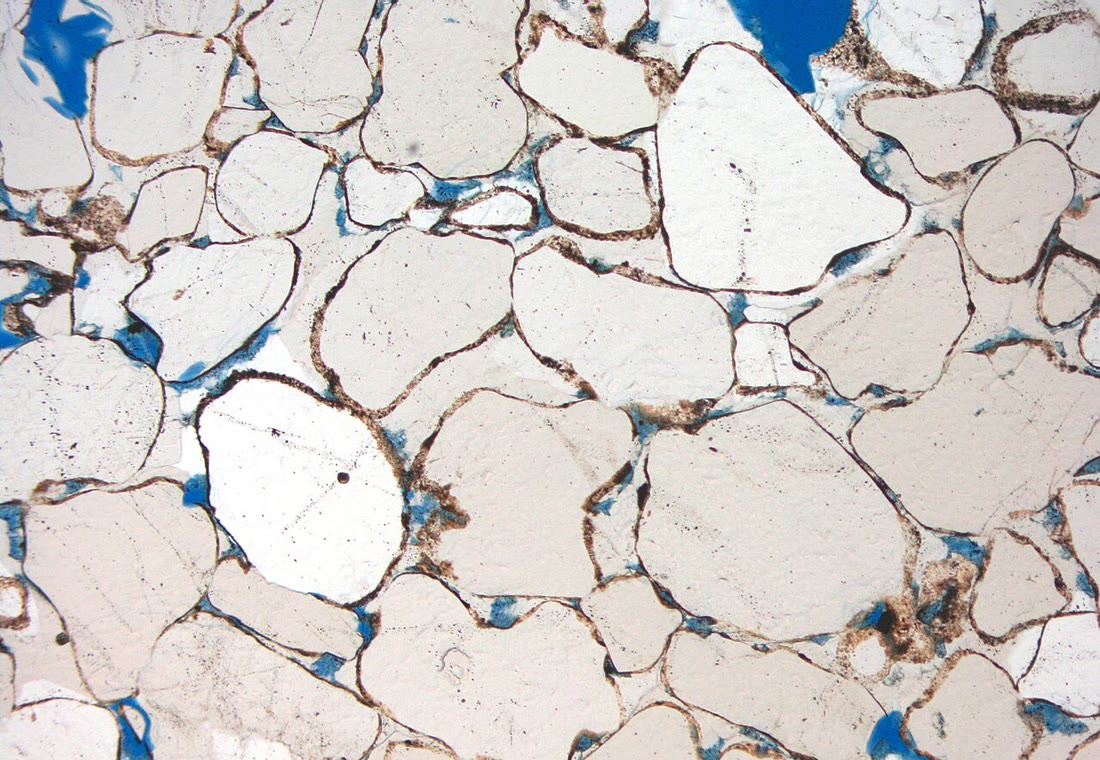
\includegraphics[width=0.62\linewidth]{images/book3/b1-quartz-overgrowths.jpg}

{\small مقطع رقيق من الحجر الرملي الكوارتزي، حجر بوتسدام الرملي (الكمبري) في ولاية نيويورك، بضوء مستقطب في مستوى واحد. تتحدّد الحبيبات الفتاتية المستديرة بحواف داكنة من الغبار والطين؛ والكوارتز الصافي خارج الحواف هو تلحيم نما على الحبيبات متّصلًا بها بصريًّا، حتى التقت النموّات المجاورة على أوجه مستقيمة. والراتنج الأزرق يملأ ما بقي من المسام. (M.~C.~Rygel, CC~BY-SA~4.0, عبر Wikimedia Commons؛ شريط المقياس الأصلي مقصوص.)}
\label{fig:b1:diagenesis-basins:overgrowths}
\end{omfigure}
% ledger: commons:potsdam

ليست كل التغيّرات تُتلف المسامية. فالماء غير المشبع \omterm{def:b1:rock-forming-minerals:mineral}{بمعدن} يذيبه: فحبيبات \omterm{def:b1:rock-forming-minerals:groups}{الفلسبار} والكربونات، والمواد اللاحمة الكربوناتية الأسبق، يمكن أن تزول وتترك مسامية ثانوية، مسامات على شكل الحبيبات التي تحلّ محلّها. \omterm{def:b1:rock-forming-minerals:mineral}{ومعادن} الطين تنمو في المسام بدورها، كأغلفة على الحبيبات أو كبلورات تملأ المسام وتضيّق الممرّات بينها، فتخفّض النفاذية. وتتغيّر \omterm{def:b1:rock-forming-minerals:mineral}{معادن} الرسوب أيضًا: فالأراغونيت في الأصداف وفي \omterm{def:b1:chemical-biogenic-sediments:factory}{مصنع الكربونات} يعود إلى الكالسيت، وهو المستقرّ عند السطح، والكالسيت في وجود ماء فيه مغنيسيوم قد يصير دولوميت.
% ledger: og:diagenesis

إحلال الكالسيت بالدولوميت، وهو الدولوميتة، تفاعل مع المغنيسيوم من الماء،
\[
  \ce{2 CaCO3 + Mg^2+ -> CaMg(CO3)2 + Ca^2+},
\]
ويغيّر حجم الصلب.

\begin{proposition}[الدولوميتة تخلق مسامية]\label{prop:b1:diagenesis-basins:dolomite}
إذا حلّ مولان من الكالسيت كثافته $\rho_c$ محلّهما مول واحد من الدولوميت كثافته $\rho_d$، ينقص حجم الصلب بالكسر
\[
  1 - \frac{M_d/\rho_d}{2M_c/\rho_c},
\]
حيث $M_c$ و$M_d$ الكتلتان المولاريتان. وب$\rho_c = \qty{2.71}{g.cm^{-3}}$ و$\rho_d = \qty{2.84}{g.cm^{-3}}$ يكون هذا الكسر \qty{12.1}{\percent}.
\end{proposition}

\begin{proof}
حجم المول \omterm{def:b1:rock-forming-minerals:mineral}{لمعدن} هو كتلته المولارية مقسومة على كثافته. يشغل مولان من الكالسيت $2M_c/\rho_c$، ومول واحد من الدولوميت $M_d/\rho_d$؛ والكسر المفقود هو واحد ناقص نسبتهما. مع $M_c = \qty{100.09}{g.mol^{-1}}$ و$M_d = \qty{184.40}{g.mol^{-1}}$ يكون الحجمان $2\times\qty{36.93}{cm^3} = \qty{73.86}{cm^3}$ و\qty{64.93}{cm^3}، و$1 - 64.93/73.86 = \num{0.121}$.
\end{proof}

وإن بقي الحجم الخارجي للصخر دون تغيير، فالصلب المفقود هو فراغ مسامي مكتسب: حجر كلسي مساميته \num{0.10}، أُحلّ محلّه بالدولوميت مولًا بمول، تصير مساميته نحو \num{0.21}. ويحتاج التفاعل إلى كمية كبيرة من المغنيسيوم، وماء البحر يحتوي منه نحو \qty{1.28}{g} لكل كيلوغرام؛ ويُفضَّل حيث تجري محاليل ملحية أو ماء البحر عبر الصخر زمنًا طويلًا (\cref{exo:b1:diagenesis-basins:12}).
% ledger: hom:calcite, webmineral:others, teos10:reference-composition, teos10:reference-salinity

يتبع \omterm{def:b1:diagenesis-basins:diagenesis}{الدياجينيز} تاريخ الرسوب. فبعد الترسيب مباشرة، قرب السطح، يكون ماء المسام ما زال ماء البحر أو البحيرة أو المطر: فتُحفر الرسوبيات بالكائنات، ويُلحم كثير منها مبكّرًا في قاع البحر أو في التربة، ويتحوّل الأراغونيت إلى كالسيت. ومع الدفن والتسخين يسود \omterm{def:b1:diagenesis-basins:compaction}{الانضغاط} والضغط الانحلالي وتلحيم الكوارتز. فإن رُفعت الحوض لاحقًا وتآكل، عاد ماء عذب من السطح إلى الصخور، فذوّب الكربونات \omterm{def:b1:rock-forming-minerals:groups}{والفلسبار} من جديد. وتسجّل \omterm{def:b1:field-lab-methods-1:thin-section}{الشريحة الرقيقة} ترتيب هذه الأحداث: \omterm{def:b1:diagenesis-basins:cement}{فالتلحيم} الذي يملأ المسام التي تركتها حبيبة مذابة أحدث من الانحلال، والنموّ الفوقي الذي كسره \omterm{def:b1:diagenesis-basins:compaction}{الانضغاط} أقدم من \omterm{def:b1:diagenesis-basins:compaction}{الانضغاط} نفسه.

\section{الأحواض الرسوبية}\label{sec:b1:diagenesis-basins:basins}

لا يتراكم الرسوب كيلومترات في السماكة إلا حيث يستمرّ القاع في \omterm{def:b1:diagenesis-basins:subsidence}{الهبوط}.

\begin{definition}[الحوض الرسوبي]\label{def:b1:diagenesis-basins:basin}
\emph{الحوض الرسوبي}\index{الحوض الرسوبي} منطقة من سطح الأرض تهبط فيها \omterm{def:b1:layered-earth:layers}{القشرة} لزمن طويل، من بضعة ملايين إلى بضع مئات الملايين من السنين، ويملأ الفراغ المتكوّن بالرسوب، بسماكة من مئات الأمتار إلى كيلومترات عديدة.
\end{definition}

\begin{definition}[الهبوط، والهبوط التكتوني]\label{def:b1:diagenesis-basins:subsidence}
\emph{الهبوط}\index{الهبوط} للحوض هو الحركة النازلة لقاعدته، أي السطح الذي ترقد عليه رسوباته، مقيسة بالنسبة إلى مرجع ثابت، كمركز الأرض. أما \emph{الهبوط التكتوني}\index{الهبوط التكتوني} فهو الجزء الناتج عن العمليات التي تصنع الحوض، متميّزًا عن الهبوط الإضافي الناجم عن وزن الرسوب والماء اللذين يملآنه؛ ويُقاس بالهبوط الذي كانت ستبلغه القاعدة تحت الماء وحده.
\end{definition}

ما يجعل القاع يهبط هو موضع الحوض في الصفيحة (الشكل أدناه).

\begin{description}
  \item[أحواض الصدوع.] الصدوع العادية تمدّد \omterm{def:b1:layered-earth:layers}{القشرة}، وتهبط كتل بينها (\cref{ch:b1:rifts-ridges-margins}). والأحواض ضيّقة وغير متماثلة، وأنصاف الخنادق تمتلئ أسرع ما يكون عند حدود صدعها. وحقول النفط في بحر الشمال توجد في بنى خندق فايكينغ وخندق الوسط، مدفونة تحت رسوبيات أحدث. وحين يتوقّف التمدّد، يبرد \omterm{def:b1:layered-earth:lithosphere}{الغلاف الصخري} الرقيق والمسخّن، ويتقلّص، ويواصل \omterm{def:b1:diagenesis-basins:subsidence}{الهبوط} ببطء، على مدى عشرات الملايين من السنين. أما وسط بحر الشمال، الذي انتهى آخر تمدّد كبير له في منتصف الكريتاسي، فقد هبط كحوض عريض على شكل صحن، امتلأ تباعًا بالطباشير، ثم بالحجارة الرملية، وعلى مدى معظم الثالث بالصخور الطينية؛ ولو حُمّل قاعه بالماء وحده لكان قد هبط \qtyrange{1100}{1400}{m} في الوسط.
  \item[الهوامش السلبية.] حيث صار الصدع محيطًا، يجعل التبريد نفسه كل هامش يهبط بعد الانفصال، وتبني إسفينة من الرسوب تزداد سماكتها نحو المحيط فوق أحواض الصدع القديمة.
  \item[أحواض الأمام الجبلي.] أمام حزام من صفائح الدفع، يثني وزن الصفائح المتراكمة \omterm{def:b1:layered-earth:lithosphere}{الغلاف الصخري} إلى أسفل، بالتوازن الإيزوستاسي، فيتكوّن حوض أعمق ما يكون عند الحزام، ويمتلئ بالحطام المتآكل منه. وأكثر صخور الكريتاسي في غرب كندا تكوّنت في مثل هذا الحوض أمام جبال روكي.
  \item[الأحواض داخل الكراتونية.] في داخل القارات القديمة، بعيدًا عن أي حدّ صفيحي، تهبط مناطق واسعة مدوّرة أو بيضاوية ببطء لأزمنة طويلة جدًّا. وحوض باريس هو مركز مثل هذا الانخفاض البنيوي، بين الكتل القديمة في بريتاني والهضبة الوسطى وفوج وآردين.
  \item[أحواض الانزياح الجانبي.] حيث يتحوّل \omterm{def:b1:faults-folds-fabrics:fault-types}{صدع انزياحي} جانبًا بالاتجاه الذي يشدّ جداره بعيدًا، أي انحناءً مُحرِّرًا، يهبط متوازي أضلاع من \omterm{def:b1:layered-earth:layers}{القشرة} بين خيطي الصدع: حوض سحبي، كتلك التي في منطقة لوس أنجلس على طول نظام سان أندرياس.
\end{description}
% ledger: ws:basins, sc80:north-sea, britannica:paris-basin

يُدرس في مجلد السنة الثانية سبب هبوط \omterm{def:b1:layered-earth:lithosphere}{الغلاف الصخري} في كل موضع، وبأيّ معدّل، وكيف تُقارن الأحواض؛ وهنا تُميَّز بمواضعها وبشكل ما تملؤه.

\begin{omfigure}
\begin{tikzpicture}[font=\scriptsize, line join=round]
% (a) rift: a half-graben
\begin{scope}
  \fill[lith granite] (0,0) -- (0,1.6) -- (1.4,1.6) -- (2.2,0.2) -- (5.0,1.0) -- (5.0,0) -- cycle;
  \fill[lith shale] (1.4,1.6) -- (2.2,0.2) -- (5.0,1.0) -- (5.0,1.6) -- cycle;
  \fill[lith sandstone] (1.4,1.6) -- (1.75,0.99) -- (5.0,1.25) -- (5.0,1.6) -- cycle;
  \draw[normal fault, thick] (1.4,1.6) -- (2.3,0.0);
  \draw[black!70] (0,1.6) -- (5.0,1.6);
  \node[anchor=south west] at (0,1.65) {(أ) صدع: نصف خندق};
  \node[fill=white, fill opacity=0.8, text opacity=1, inner sep=1pt] at (3.9,0.3) {القاعدة};
  \node[fill=white, fill opacity=0.8, text opacity=1, inner sep=1pt] at (0.65,0.8) {الجدار المرتكز};
\end{scope}
% (b) passive margin: a seaward-thickening wedge over thinned crust
\begin{scope}[xshift=6.6cm]
  \fill[lith sea] (2.0,1.6) -- (5.0,1.6) -- (5.0,0.75) -- (3.6,0.95) -- cycle;
  \fill[lith granite] (0,0) -- (0,1.2) -- (2.0,1.0) -- (3.6,0.35) -- (5.0,0.05) -- (5.0,0) -- cycle;
  \fill[lith shale] (0,1.2) -- (2.0,1.0) -- (3.6,0.35) -- (5.0,0.05) -- (5.0,0.75) -- (3.6,0.95) -- (2.0,1.6) -- (0,1.6) -- cycle;
  \draw[black!70] (0,1.6) -- (2.0,1.6) -- (3.6,0.95) -- (5.0,0.75);
  \draw[blue!60!black, thick] (2.0,1.6) -- (5.0,1.6);
  \node[anchor=south west] at (0,1.65) {(ب) هامش سلبي};
  \node[fill=white, fill opacity=0.8, text opacity=1, inner sep=1pt] at (1.0,0.45) {قشرة قارية رقيقة};
  \node[anchor=north east] at (5.0,1.58) {المحيط};
\end{scope}
% (c) foreland basin: asymmetric, deepest against the thrust belt
\begin{scope}[yshift=-3.3cm]
  \fill[lith granite] (0,0) -- (0,0.55) -- (5.0,1.35) -- (5.0,0) -- cycle;
  \fill[lith sandstone] (0,0.55) -- (5.0,1.35) -- (5.0,1.6) -- (0,1.6) -- cycle;
  \fill[lith conglomerate] (1.0,1.6) -- (3.6,1.6) -- (1.0,1.0) -- cycle;
  \fill[omLithSchist, draw=black!70] (0,0.95) -- (1.9,1.6) -- (1.3,1.95) -- (0.4,2.25) -- (0,2.3) -- cycle;
  \draw[thrust fault] (0,0.95) -- (1.9,1.6);
  \draw[thrust fault] (0,1.55) -- (1.15,1.95);
  \draw[black!70] (1.9,1.6) -- (5.0,1.6);
  \node[anchor=south west] at (2.0,1.65) {(ج) حوض أمامي جبلي};
  \node[anchor=south west, inner sep=1pt] at (0.25,2.3) {حزام الدفع};
  \node[fill=white, fill opacity=0.8, text opacity=1, inner sep=1pt] at (3.9,0.35) {القاعدة};
\end{scope}
% (d) intracratonic basin: a broad sag, layers thickening to the centre
\begin{scope}[xshift=6.6cm, yshift=-3.3cm]
  \fill[lith granite] (0,0) -- (0,1.5) .. controls (1.6,1.1) and (2.0,0.3) .. (2.5,0.3) .. controls (3.0,0.3) and (3.4,1.1) .. (5.0,1.5) -- (5.0,0) -- cycle;
  \fill[lith limestone] (0,1.5) .. controls (1.6,1.1) and (2.0,0.3) .. (2.5,0.3) .. controls (3.0,0.3) and (3.4,1.1) .. (5.0,1.5) -- (5.0,1.6) -- (0,1.6) -- cycle;
  \fill[lith shale] (0.6,1.6) .. controls (1.6,1.35) and (2.1,0.85) .. (2.5,0.85) .. controls (2.9,0.85) and (3.4,1.35) .. (4.4,1.6) -- cycle;
  \fill[lith sandstone] (1.3,1.6) .. controls (1.9,1.5) and (2.2,1.3) .. (2.5,1.3) .. controls (2.8,1.3) and (3.1,1.5) .. (3.7,1.6) -- cycle;
  \draw[black!70] (0,1.6) -- (5.0,1.6);
  \node[anchor=south west] at (0,1.65) {(د) حوض داخل كراتوني};
  \node[fill=white, fill opacity=0.8, text opacity=1, inner sep=1pt] at (4.2,0.4) {القاعدة};
\end{scope}
\end{tikzpicture}

{\small أربعة أنواع من \omterm{def:b1:diagenesis-basins:basin}{الأحواض الرسوبية} في مقطع عرضي (تخطيطي، غير متناسب، والمقياس الرأسي مبالغ فيه). (أ)~صدع: تزداد سماكة الملء عند صدع الحدّ لنصف خندق. (ب)~هامش سلبي: إسفينة من الرسوب تزداد سماكتها نحو المحيط فوق \omterm{def:b1:layered-earth:layers}{قشرة} قارية رقيقة. (ج)~حوض أمامي جبلي، أعمق ما يكون عند حزام الدفع الذي يثني وزنه القاع إلى أسفل، ويُغذّى بحطامه، وأخشن ما يكون، كونغلوميرا، قرب الحزام؛ ويتجاوز الحزام حافة حوضه. (د)~حوض داخل كراتوني: انخفاض واسع تزداد طبقاته سماكةً نحو المركز.}
\label{fig:b1:diagenesis-basins:types}
\end{omfigure}

\begin{inthefield}[كيف تُعرف الأحواض]
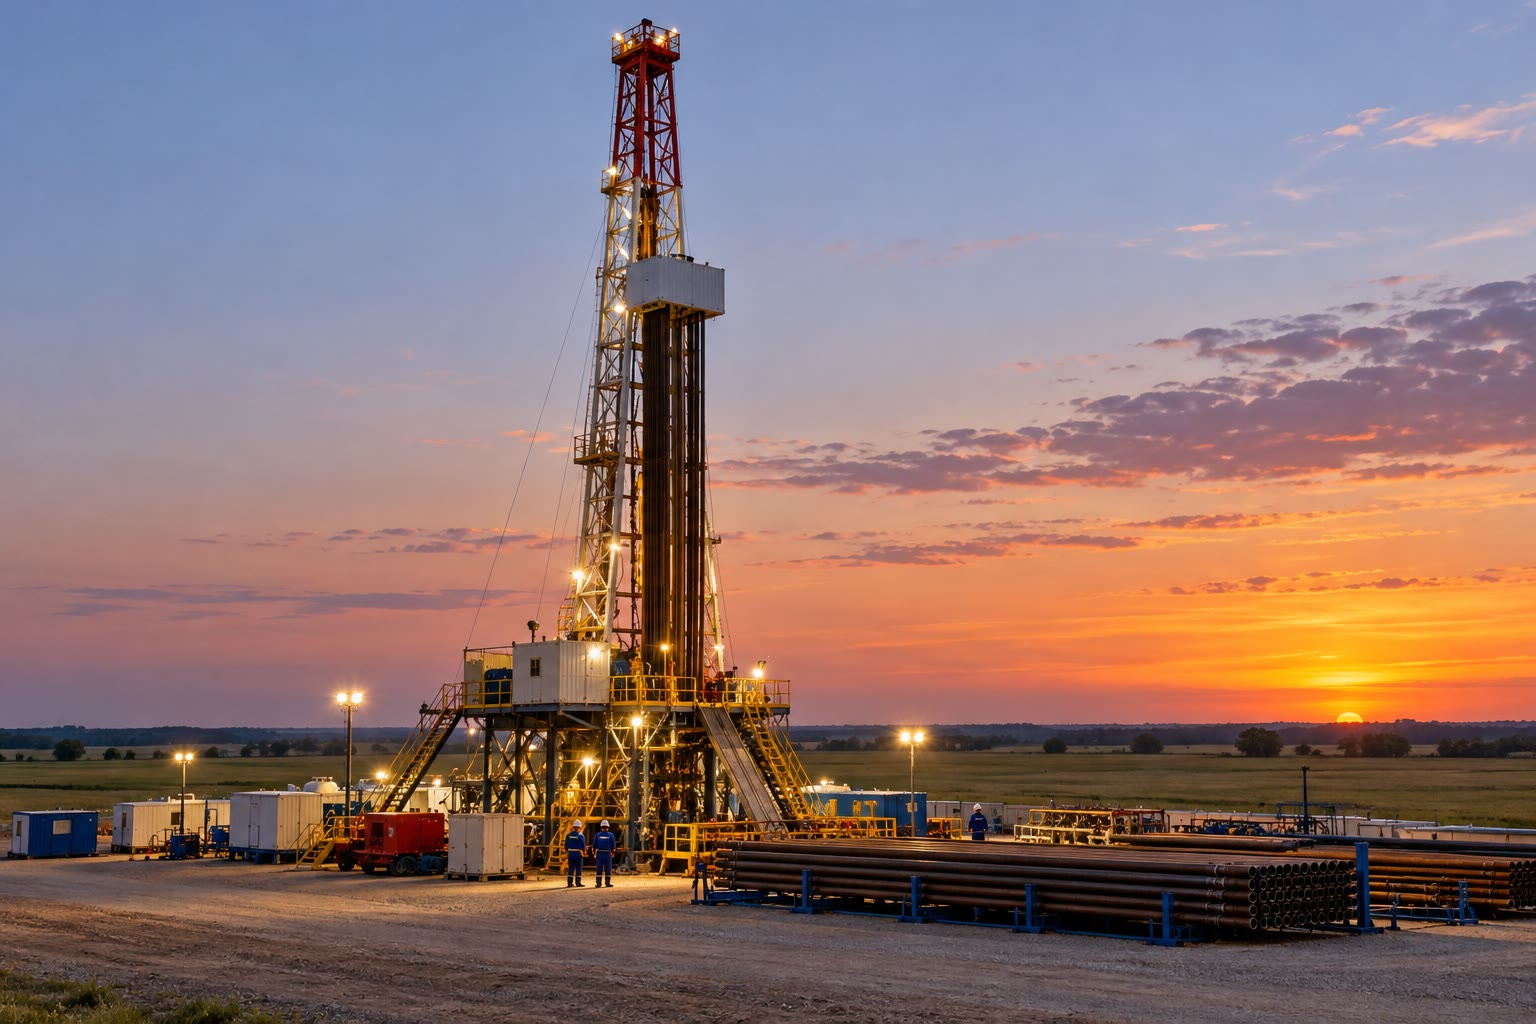
\includegraphics[width=0.3\linewidth]{images/book3/ai/b1-drilling-rig.jpg}\hfill
\begin{minipage}[b]{0.67\linewidth}
تقريبًا كل ما يُعرف عن الملء العميق لحوض يأتي من البحث عن النفط والغاز والماء. وتصوّر مسوح الانعكاس الزلزالي طبقاته وصدوعه عبر آلاف الكيلومترات المربّعة؛ والآبار تأخذ عيّنة منه عند نقطة. فالبئر يُعيد شظايا الصخر التي يقطعها الرأس، وعلى فترات لُبّات، ومنحنيات مستمرّة للخصائص الفيزيائية للصخور حول الحفرة، ومنها تُقرأ المسامية متًرًا بمتر. ومنحنيات المسامية بالعمق \omterm{prop:b1:diagenesis-basins:athy}{لقانون أثي}، وتواريخ \omterm{def:b1:diagenesis-basins:subsidence}{الهبوط} للأحواض، بُنيت أولًا من مثل هذه الآبار.
\end{minipage}

\smallskip
{\small حفّارة برّية عند الغسق، والأنابيب مكدّسة على أرفف في المقدّمة (توضيحي بالذكاء الاصطناعي).}
\end{inthefield}
% ledger: sc80:north-sea

\section{الهبوط والاستيعاب ومستوى البحر}\label{sec:b1:diagenesis-basins:accommodation}

لا يستطيع الرسوب أن يتراكم إلا حيث يتّسع المكان له تحت المستوى الذي يُنقل عنده. وفي البحر يكون هذا المستوى قريبًا من مستوى البحر، والمكان مسألة حركتين: حركة القاع، وحركة سطح البحر.

\begin{definition}[الاستيعاب]\label{def:b1:diagenesis-basins:accommodation}
\emph{الاستيعاب}\index{الاستيعاب} عند نقطة من حوض هو الفراغ المتاح لتراكم الرسوب فيها: المسافة الرأسية من قمّة الرسوب إلى مستوى البحر، قاعدة الترسيب البحري. والاستيعاب المتكوّن في فترة زمنية هو زيادة المسافة من مرجع مرتبط بالقاعدة إلى مستوى البحر.
\end{definition}

\begin{definition}[السكونية، ومستوى البحر النسبي]\label{def:b1:diagenesis-basins:eustasy}
\emph{السكونية}\index{السكونية} هي تغيّر مستوى المحيط العالمي مقيسًا بالنسبة إلى مرجع ثابت، هو مركز الأرض، وناتج عن تغيّر حجم الماء في المحيط أو حجم أحواض المحيط؛ وهي واحدة في كل مكان. و\emph{مستوى البحر النسبي}\index{مستوى البحر النسبي} في مكان ما هو ارتفاع سطح البحر فوق مرجع مرتبط بالقاعدة هناك؛ ويتغيّر بالسكونية وبالحركة الرأسية للأرض.
\end{definition}

\begin{proposition}[ميزانية الاستيعاب]\label{prop:b1:diagenesis-basins:budget}
في فترة زمنية، ليكن $\Delta E$ ارتفاع مستوى البحر السكوني، و$S$ هبوط القاعدة (وكلاهما موجب نحو الأعلى بالنسبة إلى البحر، ونحو الأسفل بالنسبة إلى القاع). \omterm{def:b1:diagenesis-basins:accommodation}{والاستيعاب} المتكوّن هو
\[
  \Delta A = \Delta E + S ,
\]
وهو يتقاسم بين سماكة الرسوب المضافة فوق المرجع، $\Delta T$، وتعمّق الماء، $\Delta W$:
$\Delta E + S = \Delta T + \Delta W$.
\end{proposition}

\begin{proof}
قِس الارتفاعات من المرجع الثابت. ليكن $e$ ارتفاع سطح البحر، و$b$ ارتفاع المرجع، و$T$ سماكة الرسوب فوق المرجع، و$W$ عمق الماء فوق الرسوب، فيكون $e = b + T + W$. \omterm{def:b1:diagenesis-basins:eustasy}{ومستوى البحر النسبي} هو $R = e - b = T + W$. وخلال الفترة، $\Delta e =
\Delta E$ و$\Delta b = -S$، ف$\Delta R = \Delta E + S$؛ و$\Delta R =
\Delta T + \Delta W$.
\end{proof}

قاع بحر يبقى عند عمق ثابت ($\Delta W = 0$) يُملأ بالسرعة نفسها التي يُخلق بها \omterm{def:b1:diagenesis-basins:accommodation}{الاستيعاب} تمامًا؛ والذي يضحل يُملأ أسرع، فيتحرّك الشاطئ نحو البحر؛ والذي يعمق يُجاع. و$\Delta T$ هو تغيّر سماكة الكومة كلّها فوق المرجع: يحسب الرسوب الجديد المرسّب، مطروحًا منه نحافة الرسوبيات الأقدم تحتها مع انضغاطها، \omterm{def:b1:diagenesis-basins:compaction}{فالانضغاط} نفسه يصنع مكانًا لرسوب أكثر (الشكل أدناه).

\begin{omfigure}
\begin{tikzpicture}[font=\footnotesize, >=Stealth]
\def\col#1#2#3#4#5{% x, datum, sediment top, sea, label
  \fill[lith granite] (#1,0.2) rectangle ++(1.4,#2-0.2);
  \fill[lith shale] (#1,#2) rectangle ++(1.4,#3-#2);
  \fill[lith sea] (#1,#3) rectangle ++(1.4,#4-#3);
  \draw[black!70] (#1,#2) -- ++(1.4,0);
  \draw[blue!60!black, thick] (#1-0.2,#4) -- ++(1.8,0);
  \node[anchor=north] at (#1+0.7,0.15) {#5};}
\draw[black!60, dash dot] (-0.6,0.9) -- (8.6,0.9) node[anchor=west, align=left] {المرجع\\ الثابت};
\col{0}{1.5}{3.0}{3.6}{الزمن $t_1$}
\col{4.4}{1.0}{3.4}{3.9}{الزمن $t_2$}
% eustasy
\draw[<->, omThm] (3.0,0.9) -- (3.0,3.6) node[midway, fill=white, inner sep=1pt] {$e_1$};
\draw[<->, omThm] (7.4,0.9) -- (7.4,3.9) node[midway, fill=white, inner sep=1pt] {$e_2$};
% subsidence of the datum
\draw[dashed, black!60] (1.4,1.5) -- (4.4,1.5);
\draw[->, thick] (4.2,1.5) -- (4.2,1.0) node[midway, anchor=east] {$S$};
% relative sea level
\draw[<->] (-0.35,1.5) -- (-0.35,3.6) node[midway, anchor=east] {$R_1$};
\draw[<->] (6.05,1.0) -- (6.05,3.9) node[midway, anchor=west] {$R_2$};
\node[anchor=west] at (1.5,2.25) {$T_1$};
\node[anchor=west] at (1.5,3.3) {$W_1$};
\node at (5.1,2.2) {$T_2$};
\node at (5.1,3.65) {$W_2$};
\node[anchor=south, align=center, blue!60!black] at (5.1,3.95) {مستوى البحر};
\node[anchor=west, align=left, font=\scriptsize] at (8.6,2.4) {$R = e - b = T + W$\\[2pt] $\Delta R = \Delta E + S$\\ $\phantom{\Delta R} = \Delta T + \Delta W$};
\end{tikzpicture}

{\small \omterm{def:b1:diagenesis-basins:accommodation}{الاستيعاب} عند مكان واحد في زمنين (تخطيطي). بين $t_1$ و$t_2$ يرتفع مستوى البحر بمقدار $\Delta E = e_2 - e_1$ فوق المرجع الثابت، ويهبط القاع بمقدار $S$: فيكبر \omterm{def:b1:diagenesis-basins:eustasy}{مستوى البحر النسبي} $R$ بمقدار $\Delta E + S$، وهو \omterm{def:b1:diagenesis-basins:accommodation}{الاستيعاب} المتكوّن، ويتقاسمه رسوب أكثر ($T_2 > T_1$) وتغيّر في عمق الماء (هنا ضحولة طفيفة، $W_2 < W_1$).}
\label{fig:b1:diagenesis-basins:accommodation}
\end{omfigure}

لا يهبط الحوض بهبوطه التكتوني وحده: فالرسوب الذي يملؤه حمل، \omterm{def:b1:layered-earth:lithosphere}{والغلاف الصخري} يهبط أكثر تحته.

\begin{proposition}[تحميل الرسوب يضخّم الهبوط]\label{prop:b1:diagenesis-basins:loading}
في توازن أيري المحلّي فوق \omterm{def:b1:layered-earth:layers}{وشاح} كثافته $\rho_m$، حوض قاعدته، محمّلة بالماء ذي الكثافة $\rho_w$ وحده، تقع على العمق $Y$ تحت مستوى البحر، تحتوي، حين يُملأ حتى مستوى البحر برسوب متوسط كثافته $\rho_s$، السماكة
\[
  h = Y\,\frac{\rho_m - \rho_w}{\rho_m - \rho_s}
\]
من الرسوب. وعلى اليابسة، حين يُملأ حتى مستوى المحيط بالهواء فوقه، يكون المعامل $\rho_m/(\rho_m - \rho_s)$.
\end{proposition}

\begin{proof}
قارن العمودين تحت \omterm{def:b1:layered-earth:lithosphere}{الغلاف الصخري} نفسه، كتلته $M$ لكل وحدة مساحة وسماكته $L$، حتى عمق تعويض $z_c$ تحتهما معًا. والعمود المحمّل بالماء يحوي $\rho_w Y + M + \rho_m(z_c - Y - L)$؛ والعمود المملوء بالرسوب $\rho_s h + M + \rho_m(z_c - h - L)$. وب\cref{prop:b1:isostasy-gravity:equal-mass} تتساوى الكتلتان، ف$\rho_w Y - \rho_m Y = \rho_s h - \rho_m h$، أي $h(\rho_m - \rho_s) =
Y(\rho_m - \rho_w)$. ومع الهواء بدل الماء، يُستبدل $\rho_w$ بالصفر.
\end{proof}

ب$\rho_m = \qty{3300}{kg.m^{-3}}$، و$\rho_w = \qty{1030}{kg.m^{-3}}$، ورسوب متوسط كثافته \qty{2300}{kg.m^{-3}}، يكون المعامل $2270/1000 = \num{2.27}$: حوض يتيح مكانًا ل\qty{1}{km} من الماء بهبوطه التكتوني، يحتوي \qty{2.27}{km} من الرسوب. وعلى اليابسة يكون المعامل $3300/1000 = \num{3.3}$. وكثافة الملء ليست ثابتة: فهي تزداد مع انضغاط الرسوب، ويزداد المعامل معها، فتحويل سماكة الرسوب إلى هبوط تكتوني يقتضي فكّ انضغاط كل طبقة، خطوةً زمنية بعد أخرى. وذلك الإجراء، أي الإزالة المتتابعة للطبقات، يخصّ مجلد السنة الثانية.

ومستوى البحر نفسه بعيد عن الثبات. ففي أقصى العصر الجليدي الأخير، غطّت صفائح الجليد معظم أمريكا الشمالية وشمال أوروبا، وكان الماء المحبوس فيها قد أُخذ من المحيط. ومصحَّحةً لاستجابة الأرض الصلبة للأحمال المتغيّرة من الجليد والماء، تعطي مشاهدات الشواطئ القديمة مستوى بحر هبط بسرعة بنحو \qty{40}{m} قبل نحو \num{30000} سنة، ثم ببطء إلى \qty{134}{m} تحت مستوى اليوم، من \qtyrange{29}{21}{\ka}؛ وكان الجليد المستقرّ على اليابسة حينئذٍ يحوي نحو \qty{52e6}{km^3} أكثر مما اليوم. والرقم \qty{125}{m} الذي يُذكر كثيرًا أصغر، لأنه غالبًا لا يُصحَّح لهذه الآثار الإيزوستاسية. وجاء انحسار الجليد أساسًا بين نحو \qty{16.5}{\ka} و\qty{8.2}{\ka}، بمتوسط \qty{12}{m} لكل ألف سنة، وب\qty{40}{mm} في السنة أو أكثر بين \qty{14.5}{\ka} و\qty{14.0}{\ka}.
% ledger: lambeck:lgm, lambeck:deglaciation

وتُقرأ مستويات البحر المنخفضة الأقدم من نظائر الأكسجين في فورامينيفيرا من لُبّات أعماق البحار، التي تسجّل حجم الجليد على اليابسة. وبتكديس سبع إعادات بناء من هذا النوع عبر آخر \num{430000} سنة، وخمس عبر آخر \num{800000}، تتوازن أخطاء كلٍّ منها؛ ومقاسًا إلى الهولوسين وإلى أدنى انخفاض للبحر في العصر الجليدي الأخير، يحمل التكديس عدم يقين قدره \qtyrange{9}{12}{m} (الشكل أدناه). وهو يُظهر الدورات الجليدية كمنشار: هبوطات بطيئة لمستوى البحر، تنتهي كلّ منها بارتفاع سريع، خمس مرّات في آخر \num{800000} سنة، ارتفاع أكثر من \qty{100}{m} في أقلّ من \num{20000} سنة. \omterm{def:b1:diagenesis-basins:eustasy}{والسكونية} على هذا المقياس تحرّك الشاطئ ذهابًا وإيابًا عبر الرفوف القارية.
% ledger: spratt:stack, data:b3-sealevel-stack

\begin{omfigure}
\begin{tikzpicture}[font=\footnotesize]
\begin{axis}[width=16cm, height=4.8cm, xmin=0, xmax=800, ymin=-150, ymax=40,
    x dir=reverse, xlabel={العمر (آلاف السنين قبل الحاضر)}, xlabel style={yshift=2pt},
    ylabel={مستوى البحر (m)}, ytick={-150,-100,-50,0},
    title={(أ) آخر \num{800000} سنة (خمسة سجلّات)}, title style={font=\footnotesize},
    axis on top]
  \addplot[draw=none, name path=hi] table[x=age, y=hi] {figdata/out/bachelor-1-sea_level-long.dat};
  \addplot[draw=none, name path=lo] table[x=age, y=lo] {figdata/out/bachelor-1-sea_level-long.dat};
  \addplot[omThm!25] fill between[of=hi and lo];
  \addplot[thin, omThm] table[x=age, y=sl] {figdata/out/bachelor-1-sea_level-long.dat};
  \draw[black!50, densely dotted] (axis cs:0,0) -- (axis cs:800,0);
\end{axis}
\end{tikzpicture}

\medskip
\begin{tikzpicture}[font=\footnotesize]
\begin{axis}[width=16cm, height=4.8cm,
    xmin=0, xmax=140, ymin=-160, ymax=40, x dir=reverse,
    xlabel={العمر (آلاف السنين قبل الحاضر)}, ylabel={مستوى البحر (m)},
    ytick={-150,-100,-50,0},
    title={(ب) آخر \num{140000} سنة (سبعة سجلّات)}, title style={font=\footnotesize},
    axis on top]
  \addplot[draw=none, name path=hi] table[x=age, y=hi] {figdata/out/bachelor-1-sea_level-short.dat};
  \addplot[draw=none, name path=lo] table[x=age, y=lo] {figdata/out/bachelor-1-sea_level-short.dat};
  \addplot[omThm!25] fill between[of=hi and lo];
  \addplot[thick, omThm] table[x=age, y=sl] {figdata/out/bachelor-1-sea_level-short.dat};
  \draw[black!50, densely dotted] (axis cs:0,0) -- (axis cs:140,0);
  \addplot[only marks, mark=*, mark size=1.6pt, black] coordinates {(21,-134)};
  \draw[black!60, thin] (axis cs:21,-131) -- (axis cs:21,-46);
  \node[anchor=south, font=\scriptsize, fill=white, inner sep=1pt] at (axis cs:36,-46) {\qty{-134}{m} عند \qty{21}{\ka} من الشواطئ القديمة (Lambeck et al.\ 2014)};
\end{axis}
\end{tikzpicture}

{\small مستوى البحر العالمي بالنسبة إلى اليوم، من تكديس Spratt and Lisiecki (2016): المكوّن الرئيسي الأول لخمس إعادات بناء من لُبّات أعماق البحار عبر \num{800000} سنة (أ)، ولسبع منها عبر آخر \num{140000} (ب)، مع نطاق الانحراف المعياري الواحد. وأدنى قيمة في التكديس، \qty{-130}{m} عند \qty{24}{\ka}، تقع داخل ذلك النطاق من القيمة \qty{-134}{m} المستخلصة من الشواطئ القديمة (النقطة)؛ وتقف قمّة آخر فترة دفء بين جليدية نحو \qty{3}{m} فوق اليوم عند \qty{121}{\ka}. البيانات: NOAA NCEI World Data Service for Paleoclimatology.}
\label{fig:b1:diagenesis-basins:sea-level}
\end{omfigure}
% computed in figdata/bachelor-1/sea_level.py; ledger: data:b3-sealevel-stack, spratt:stack, lambeck:lgm

خلال عمر حوض تكون هذه التأرجحات قصيرة. فهبوط جليدي يزيد على \qty{100}{m} في بضعة عشرات الآلاف من السنين سريع وكبير مقارنةً \omterm{def:b1:diagenesis-basins:subsidence}{بالهبوط التكتوني}، الذي لا يبلغ كيلومترًا أو أكثر إلا على مدى عشرات الملايين من السنين؛ لكن التأرجحات الجليدية تبقى ضمن مدى قدره نحو \qty{150}{m}، فيصنع \omterm{def:b1:diagenesis-basins:subsidence}{الهبوط} في الملء السميك لحوض معظم المكان، وتضبط \omterm{def:b1:diagenesis-basins:eustasy}{السكونية} إيقاع طبقاته.
% ledger: data:b3-sealevel-stack, sc80:north-sea

\section{التمارين}

\begin{exercise}[$\star$]\label{exo:b1:diagenesis-basins:1}
باستعمال معاملات \cref{tab:b1:diagenesis-basins:athy}، احسب مسامية الحجر الرملي والصخر الطيني عند \qty{2000}{m}. وعلى أيّ عمق انخفضت مسامية كل منهما إلى نصف قيمتها السطحية؟
% ledger: pybacktrack:compaction
\end{exercise}

\begin{exercise}[$\star$]\label{exo:b1:diagenesis-basins:2}
خلال فترة زمنية يرتفع مستوى البحر ب\qty{30}{m} \omterm{def:b1:diagenesis-basins:eustasy}{بالسكونية}، ويهبط قاعدة رفّ بمقدار \qty{50}{m}، ويُضاف \qty{60}{m} من الرسوب فوق مرجع على القاعدة. باستعمال \cref{prop:b1:diagenesis-basins:budget}، احسب \omterm{def:b1:diagenesis-basins:accommodation}{الاستيعاب} المتكوّن وتغيّر عمق الماء. هل يتعمّق الرفّ أم يضحل؟
\end{exercise}

\begin{exercise}[$\star$]\label{exo:b1:diagenesis-basins:3}
يحتاج هبوط تكتوني لحوض إلى مكان ل\qty{1.0}{km} من الماء. مع $\rho_m = \qty{3300}{kg.m^{-3}}$ و$\rho_w = \qty{1030}{kg.m^{-3}}$، كم سماكة الرسوب الذي يملؤه حتى مستوى البحر إن كانت كثافته المتوسطة \qty{2300}{kg.m^{-3}}؟ و\qty{2500}{kg.m^{-3}}؟ ولماذا يعطي الملء الأكثف سماكة أكبر؟
\end{exercise}

\begin{exercise}[$\star$]\label{exo:b1:diagenesis-basins:4}
للكالسيت الكتلة المولارية \qty{100.09}{g.mol^{-1}} والكثافة \qty{2.71}{g.cm^{-3}}؛ وللدولوميت \qty{184.40}{g.mol^{-1}} و\qty{2.84}{g.cm^{-3}}. (أ)~احسب الحجم المولاري لكل منهما. (ب)~بأيّ كسر يتغيّر حجم الصلب حين يصير مولان من الكالسيت مولًا واحدًا من الدولوميت؟ (ج)~حجر كلسي مساميته \num{0.10} يُحوَّل إلى دولوميت مولًا بمول دون تغيّر حجمه الخارجي. ما مساميته الجديدة؟
% ledger: hom:calcite, webmineral:others
\end{exercise}

\begin{exercise}[$\star\star$]\label{exo:b1:diagenesis-basins:5}
يشغل صخر طيني أعلى \qty{1000}{m} من حوض. (أ)~احسب سماكته الصلبة ومسامّيته المتوسطة. (ب)~يُدفن حتى تقع قمّته على \qty{2000}{m}. باستعمال \cref{met:b1:diagenesis-basins:decompaction}، لكن بنقل القمّة إلى الأسفل بدلًا من الأعلى، أوجد سماكته الجديدة ومسامّيته المتوسطة. (ج)~كم من الماء طرد كل متر مربّع من الصخر الطيني؟
% ledger: pybacktrack:compaction
\end{exercise}

\begin{exercise}[$\star\star$]\label{exo:b1:diagenesis-basins:6}
يقع حجر رملي بين \qty{2500}{m} و\qty{2800}{m}. (أ)~احسب سماكته الصلبة. (ب)~افكّ انضغاطه إلى السطح ب\cref{met:b1:diagenesis-basins:decompaction}، مدوّنًا كل خطوة من خطوات نيوتن ابتداءً من $b_0 = \qty{300}{m}$. (ج)~بأيّ عامل نحّفه الدفن؟
% ledger: pybacktrack:compaction
\end{exercise}

\begin{exercise}[$\star\star$]\label{exo:b1:diagenesis-basins:7}
في أقصى العصر الجليدي الأخير احتوى الجليد المستقرّ على اليابسة نحو \qty{52e6}{km^3} أكثر مما اليوم. خذ كثافة الجليد \qty{916.7}{kg.m^{-3}}، وكثافة ماء الذوبان \qty{1000}{kg.m^{-3}}، ومساحة محيط اليوم \qty{361.84e6}{km^2}. (أ)~أيّ انخفاض لمستوى البحر يمثّله هذا الجليد؟ (ب)~قارنه ب\qty{134}{m} المستخلصة من الشواطئ القديمة. (ج)~أيّ مساحة محيط تعطي بالضبط \qty{134}{m}، ولماذا كان محيط العصر الجليدي أصغر؟
% ledger: lambeck:lgm, iapws:ice-density, charette:ocean-volume
\end{exercise}

\begin{exercise}[$\star\star$]\label{exo:b1:diagenesis-basins:8}
يعطي تكديس مستوى البحر \qty{-98.1}{m} عند \qty{16}{\ka} و\qty{-9.1}{m} عند \qty{8}{\ka}. (أ)~احسب متوسط معدّل الارتفاع بالأمتار لكل ألف سنة، وقارنه ب\qty{12}{m} لكل ألف سنة المستخلصة من الشواطئ القديمة لانحسار الجليد الرئيسي. (ب)~بين \qty{14.5}{\ka} و\qty{14.0}{\ka} ارتفع مستوى البحر بمعدّل \qty{40}{mm} في السنة أو أكثر. كم مرّة يزيد ذلك على المتوسط، وكم ارتفع مستوى البحر في تلك الخمسمئة سنة؟
% ledger: data:b3-sealevel-stack, lambeck:deglaciation
\end{exercise}

\begin{exercise}[$\star\star$]\label{exo:b1:diagenesis-basins:9}
يقع رفّ تحت \qty{20}{m} من الماء. وقاعه يهبط بمعدّل \qty{50}{m} لكل مليون سنة. (أ)~على مدى مليوني سنة ينخفض مستوى البحر ب\qty{40}{m} \omterm{def:b1:diagenesis-basins:eustasy}{بالسكونية}، بينما يبقى عمق الماء كما هو. كم استيعاب يتكوّن، وكم رسوب يُضاف؟ (ب)~ثم ينخفض مستوى البحر ب\qty{120}{m} في \num{20000} سنة، عند بداية تجمّد، ولا يُضاف رسوب. على أيّ ارتفاع فوق مستوى البحر يقف قاع البحر السابق في النهاية؟
\end{exercise}

\begin{exercise}[$\star\star\star$]\label{exo:b1:diagenesis-basins:10}
(أ)~بيّن أن طبقة سماكتها $h$ على العمق $z$، رقيقة بالقياس إلى طول الاضمحلال $\lambda$، تكون سماكتها عند إعادتها إلى السطح $h_0 \approx h\,(1 - \varphi(z))/(1 -
\varphi_0)$. (ب)~طبّقه على \qty{10}{m} من صخر طيني على \qty{3000}{m}، وقارنه \omterm{def:b1:diagenesis-basins:compaction}{بفكّ الانضغاط} الدقيق، أي \qty{23.1}{m}. (ج)~لماذا يكون التقريب كبيرًا قليلًا أكثر مما ينبغي؟
% ledger: pybacktrack:compaction
\end{exercise}

\begin{exercise}[$\star\star\star$]\label{exo:b1:diagenesis-basins:11}
يُملأ حوض حتى مستوى البحر ب\qty{3000}{m} من الصخر الطيني، مضغوطًا \omterm{prop:b1:diagenesis-basins:athy}{بقانون أثي}، ومساماته مملوءة بماء كثافته \qty{1030}{kg.m^{-3}}. (أ)~احسب المسامية المتوسطة والكثافة المتوسطة للملء. (ب)~باستعمال \cref{prop:b1:diagenesis-basins:loading} و$\rho_m =
\qty{3300}{kg.m^{-3}}$، احسب معامل التحميل \omterm{def:b1:diagenesis-basins:subsidence}{والهبوط} المحمّل بالماء الذي يمثّله الملء. (ج)~لماذا يعطي أخذ كثافة الحبيبات، \qty{2700}{kg.m^{-3}}، معاملًا أكبر بكثير، ولماذا يكون ذلك خطأً؟
% ledger: pybacktrack:compaction
\end{exercise}

\begin{exercise}[$\star\star\star$]\label{exo:b1:diagenesis-basins:12}
يجب أن يُحوَّل مكعب من متر مكعب من حجر كلسي مساميته \num{0.10} إلى دولوميت بالكامل، مولًا بمول. يحتوي ماء البحر \qty{35.165}{g} من الملح لكل كيلوغرام، منه كسر كتلي \num{0.0365} ماغنيسيوم (\qty{24.305}{g.mol^{-1}}). (أ)~كم مولًا من الكالسيت يحتوي المكعب (بالحجم المولاري من \cref{exo:b1:diagenesis-basins:4})؟ (ب)~كم مولًا من الماغنيسيوم يحتاج التفاعل؟ (ج)~ما الكتلة والحجم من ماء البحر (\qty{1030}{kg.m^{-3}}) الذي يجب أن يجري عبر المكعب إن أعطى كل ماغنيسيومه؟ (د)~ماذا يقول الجواب عن مكان تكوّن الدولوميت؟
% ledger: teos10:reference-composition, teos10:reference-salinity, hom:calcite
\end{exercise}

\section{مسألة: فكّ انضغاط ملء حوض}

\begin{problem}[{مسألة نهاية الأسبوع --- كم كانت سماكة رسوبيات بئر حين رُسّبت، وكيف صُنع لها المكان}]
\label{pb:b1:diagenesis-basins:1}
% values: calc/ch23.py; the well, its units, ages and the eustatic changes are invented
بئر محفور على سهل ساحلي، عند مستوى البحر، يخترق ثلاث وحدات قبل أن يصل إلى القاعدة عند \qty{3200}{m}:
\begin{center}
\begin{tabular}{llll}
\hline
الوحدة & الصخر & العمق اليوم (m) & زمن الترسيب \\
\hline
1 & حجر رملي & 0--800     & \qtyrange{15}{0}{\Ma} \\
2 & صخر طيني     & 800--2600  & \qtyrange{55}{15}{\Ma} \\
3 & طباشير     & 2600--3200 & \qtyrange{75}{55}{\Ma} \\
\hline
\end{tabular}
\end{center}
خذ معاملات \cref{tab:b1:diagenesis-basins:athy}، وكثافة ماء المسام \qty{1030}{kg.m^{-3}}، و$g = \qty{9.81}{m.s^{-2}}$، وافترض أن كل وحدة انضغطت \omterm{prop:b1:diagenesis-basins:athy}{بقانون أثي}، وماؤها حرّ في الهروب، طوال تاريخها. وتُظهر الكائنات الدقيقة المتحجّرة أن الماء كان ضحلًا، وبالعمق نفسه، في بداية كل فترة ونهايتها.

\medskip
\noindent\textbf{الجزء الأول --- العمود اليوم.}
\begin{enumerate}
  \item احسب المسامية عند قمّة كل وحدة وعند قاعدتها.
  \item احسب المسامية المتوسطة لكل وحدة.
  \item كم من الماء تحوي كل وحدة تحت متر مربّع واحد؟
  \item احسب الكثافة الحجمية لكل وحدة، مشبعةً بالماء، والكثافة المتوسطة للعمود كلّه.
  \item احسب الضغطين الصخري والهيدروستاتيكي عند قاعدة العمود، \omterm{def:b1:stress-strain-rheology:lithostatic}{والإجهاد الفعّال} هناك.
  \item على أيّ عمق تتساوى مسامية الحجر الرملي والصخر الطيني؟ وأيّهما أكثر مسامية تحته؟
\end{enumerate}

\noindent\textbf{الجزء الثاني --- الحبيبات.}
\begin{enumerate}[resume]
  \item احسب السماكة الصلبة لكل وحدة.
  \item ما السماكة الصلبة للعمود كلّه؟ وما الكسر من عمود اليوم الذي هو ماء؟
  \item احسب لكل وحدة معدّل تراكم الحبيبات، بالأمتار من الصلب لكل مليون سنة.
  \item أيّ وحدة كان إمداد حبيباتها أسرع؟ وأيّها أبطأ؟
\end{enumerate}

\noindent\textbf{الجزء الثالث --- الوحدات كما رُسّبت.}
\begin{enumerate}[resume]
  \item كم كانت سماكة الحجر الرملي حين رُسّب؟ ولماذا لا يحتاج الأمر إلى حساب؟
  \item افكّ انضغاط الصخر الطيني إلى السطح: كم كانت سماكته عند \qty{15}{\Ma}، حين انتهى ترسيبه لتوّه؟
  \item افكّ انضغاط الطباشير إلى السطح: كم كانت سماكته عند \qty{55}{\Ma}؟
  \item كم كانت سماكة الطباشير عند \qty{15}{\Ma}، مدفونًا تحت الصخر الطيني في السؤال السابق؟
  \item ما سماكة العمود كلّه فوق القاعدة عند \qty{55}{\Ma} وعند \qty{15}{\Ma}؟
  \item احسب معدّل الترسيب لكل وحدة من سماكتها اليوم، ومن سماكتها عند الترسيب. أيّهما ذو معنى؟
  \item بأيّ كسر ترقّق الصخر الطيني منذ \qty{15}{\Ma}؟
\end{enumerate}

\noindent\textbf{الجزء الرابع --- صنع المكان.}
\begin{enumerate}[resume]
  \item خذ أعلى القاعدة مرجعًا. باستعمال \cref{prop:b1:diagenesis-basins:budget}، احسب \omterm{def:b1:diagenesis-basins:accommodation}{الاستيعاب} المتكوّن من \qtyrange{75}{55}{\Ma}، ومن \qtyrange{55}{15}{\Ma}، ومن \qty{15}{\Ma} حتى اليوم.
  \item تعطي منحنى سكونية للمنطقة مستوى بحر أعلى ب\qty{60}{m} عند \qty{55}{\Ma} منه عند \qty{15}{\Ma}، وأعلى ب\qty{30}{m} عند \qty{15}{\Ma} منه اليوم (قيم مفترضة). احسب هبوط القاعدة في الفترتين الأخيرتين.
  \item احسب متوسط معدّل \omterm{def:b1:diagenesis-basins:subsidence}{الهبوط} في كل منهما، بالأمتار لكل مليون سنة.
  \item أيّ حصّة من \omterm{def:b1:diagenesis-basins:subsidence}{الهبوط} كان على \omterm{def:b1:diagenesis-basins:eustasy}{السكونية} أن تعوّض في كل فترة؟ وهل ساعدت \omterm{def:b1:diagenesis-basins:eustasy}{السكونية} ملء الحوض أم أعاقته؟
  \item من \omterm{def:b1:diagenesis-basins:accommodation}{الاستيعاب} الذي امتلأ منذ \qty{15}{\Ma}، كم صنعه انضغاط الصخر الطيني والطباشير تحته؟
  \item لماذا لا يمكن قراءة هبوط القاعدة من سماكة العمود اليوم؟
  \item ما سماكة وحدة الصخر الطيني حين رُسّبت؟
\end{enumerate}
\end{problem}
